\documentclass{article}
 
\usepackage{color}
\usepackage{listings}
\usepackage{graphicx}
\usepackage{subfig}

\definecolor{MyYellow}{rgb}{1,1,0.8}
 
\lstset{language=Matlab,backgroundcolor=\color{MyYellow},basicstyle=\footnotesize,numberstyle=\footnotesize,numbers=left,stepnumber=1,numbersep=5pt,breaklines=true,frame=lines,tabsize=2}
 
\author{Ruurd Moelker \and Jan Paul Posma}
\date{\today}
\title{Signalen \& Systemen \\Practicum 3}

\begin{document}
\maketitle
 
\section{Opgave 1}
Om de convolutie in matlab te bepalen gebruiken wij het commando:
$conv(xx,~[1,~-0.9])$
De filterco\"efici\"enten zijn hierbij 1 en 0.9.

Het invoersignaal $x[n]$ is de reeks van getallen startende met 10 maal 256 gevolgd door 40 maal een 0 waarna de reeks zich herhaald tot 100 getallen zijn bereikt.

\section{Opgave 2}
De stemplot van x[n] in te zien samen met de stemplot van w[n] in figuur \ref{fig:opgave2}.

\begin{figure}[h]
  \centering
 	\subfloat[][x[n]]{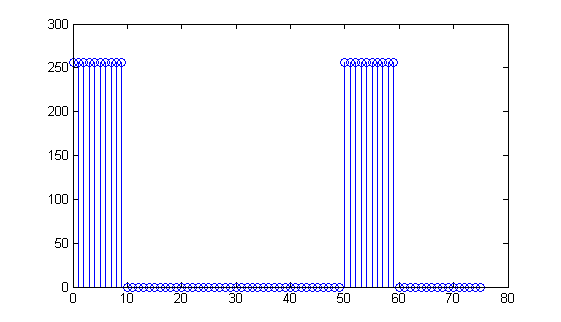
\includegraphics[width=0.4\textwidth]{content/2xx.png}}
	\subfloat[][w[n]]{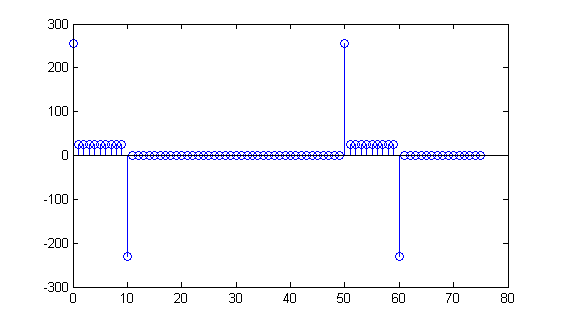
\includegraphics[width=0.4\textwidth]{content/2ww.png}}
  \caption{Stemplot van x[n] en w[n] over het interval 0 \lte n \lte 75}
  \label{fig:opgave2}
\end{figure}

\section{Opgave 3}
Het matlab commando $length()$ geeft de lengte van een signaal. Voor x[n] is deze lengte 101 en voor w[n] is de lengte 102. De lengte van de convolutie wordt inderdaad bepaald door $length(xx)+length(bb)-1$ waarbij bb de vector met co\"efficienten is, in dit geval [1, -0.9], dus lengte 2.

\section{Opgave 4}
$r = 0.9$
$M = 22$
$rr = r .^ (0:M)$
$yy = conv(ww, rr)$

\section{Opgave 5}
In figuur \ref{fig:opgave5} is de benadering van $x[n]$ door de convolutie van de reeks $rr$ op $w[n]$ geplot in een stem grafiek.
\begin{figure}[h]
  \centering
 	\subfloat[][w[n]]{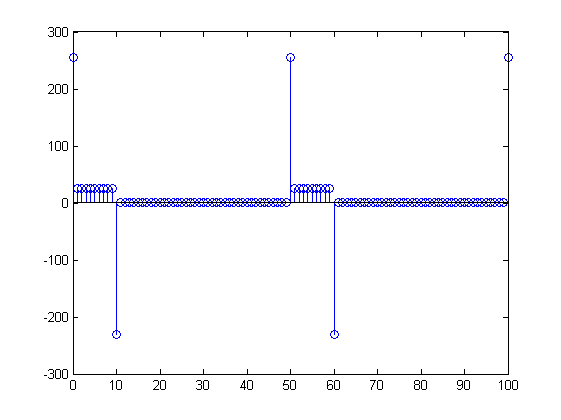
\includegraphics[width=0.4\textwidth]{content/5ww.png}}
	\subfloat[][y[n]]{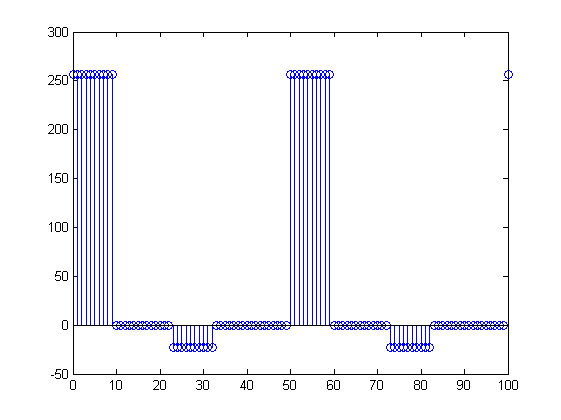
\includegraphics[width=0.4\textwidth]{content/5yy.png}}
  \caption{Stemplot van w[n] en de benadering van w[n] van x[n]}
  \label{fig:opgave5}
\end{figure}

\section{Opgave 6}
In figuur \ref{fig:opgave6}
\begin{figure}[h]
  \centering
 	\subfloat[][x[n]]{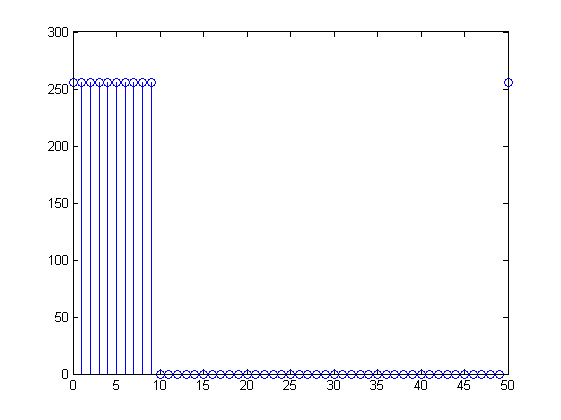
\includegraphics[width=0.4\textwidth]{content/6xx.png}}
	\subfloat[][y[n]]{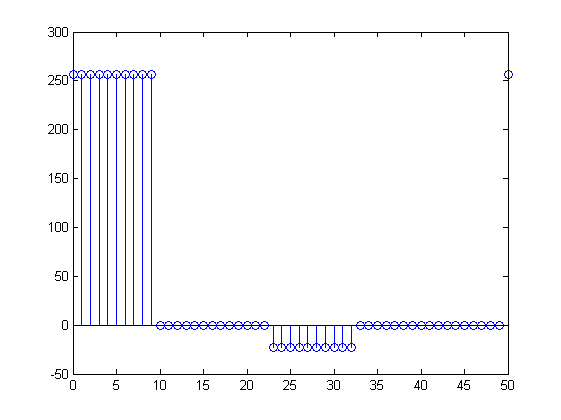
\includegraphics[width=0.4\textwidth]{content/6yy.png}}
	\subfloat[][x[n]-y[n]]{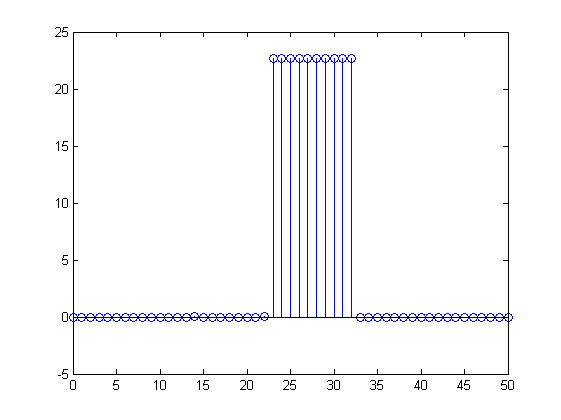
\includegraphics[width=0.4\textwidth]{content/6.png}}
  \caption{!!!!!!!!!}
  \label{fig:opgave6}
\end{figure}

\section{Opgave 7}
De waarde van r wordt bepaald door de sterkte die we aan de echo toekennen, het is immers de amplitude van het signaal P tijdeenheden terug dus: $r = 0.9$. P is de tijdverschuiving van de echo uigedrukt in tijdseenheden van de sample frequentie dus $p = \delta~t*f_s = 8000 * 0.2 = 1600$.

\section{Opgave 8}
De echo van een signaal kan met een FIR filter met convolutie $[1, 0_1 .. 0_p-1, 0.9]$ gemaakt worden. In matlab wordt het nieuwe signaal yy uit bronsignaal x2 berekend: $yy = conv(x2, [1 zeros(1,8000*0.2 - 1) 0.9]);$. Het oorspronkelijke signaal x2 en gefilterd signaal yy zijn uitgezet in figuur \ref{fig:opgave8}.
\begin{figure}[h]
  \centering
 	\subfloat[][x2[n]]{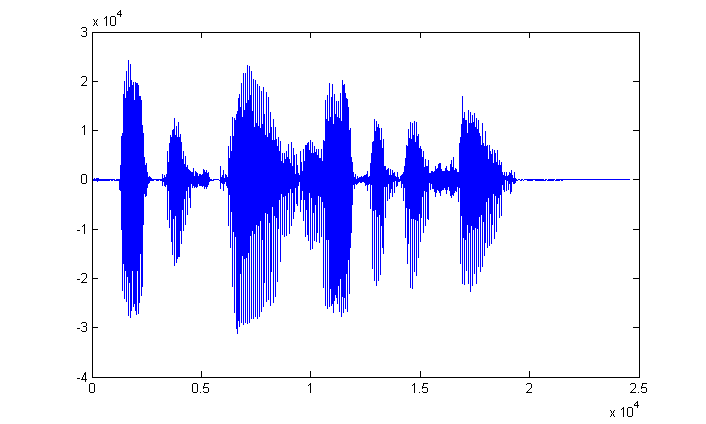
\includegraphics[width=0.4\textwidth]{content/8x2.png}}
	\subfloat[][yy[n]]{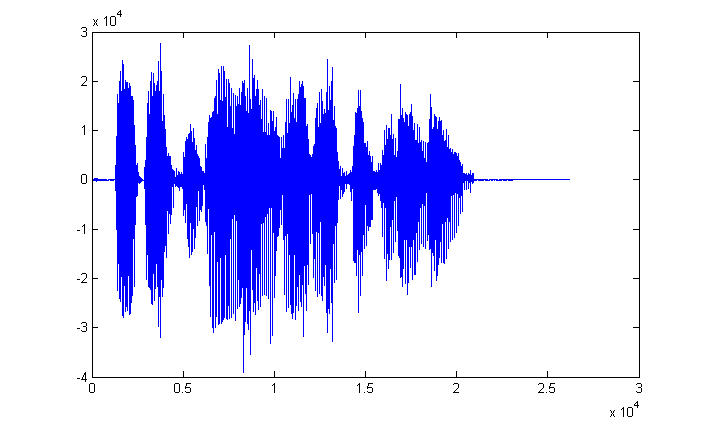
\includegraphics[width=0.4\textwidth]{content/8yy.png}}
  \caption{Het orginele signaal x2 verkregen uit functie labdat.mat en het signaal met echo yy}
  \label{fig:opgave8}
\end{figure}
%\begin{figure}[h]
 % \centering
 % \subfloat[][$I_0 = 1$]{\label{fig:b1i1}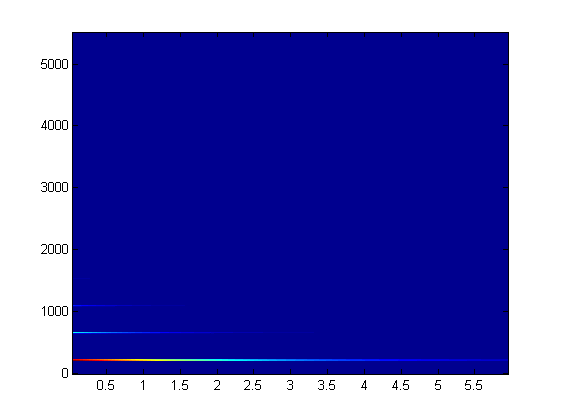
\includegraphics[width=0.4\textwidth]{content/b1i1.png}}                
  %\subfloat[][$I_0 = 5$]{\label{fig:b1i5}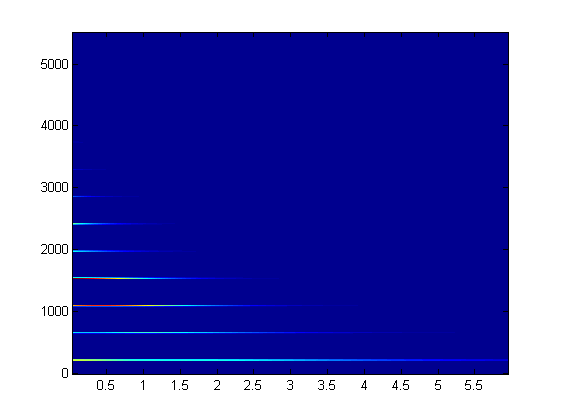
\includegraphics[width=0.4\textwidth]{content/b1i5.png}}
  %\subfloat[][$I_0 = 10$]{\label{fig:b1i10}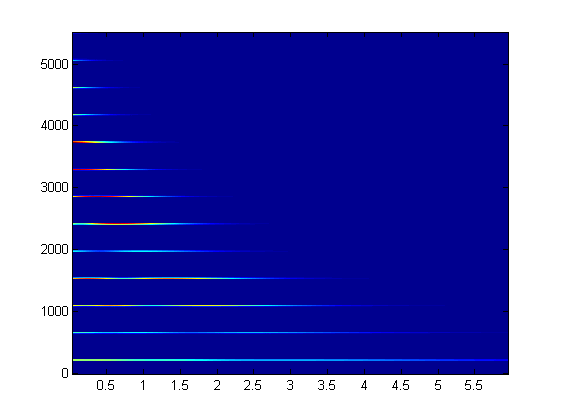
\includegraphics[width=0.4\textwidth]{content/b1i10.png}}
 % \caption{Geval 1 met verschillende $I_0$ waardes}
 % \label{fig:case1b}
%\end{figure}




In dit practicum worden geluiden geproduceerd met behulp van frequentiemodulatie volgens de functie:
$$x(t) = A(t)cos(2 \pi f_c t + I(t)cos(2 \pi f_m t + \phi_m) + \phi_c)$$
$A(t)$ en $I(t)$ worden gegeven door middel van:
$$A(t) = A_0~exp(\frac{-t}{\tau})$$
$$I(t) = I_0~exp(\frac{-t}{\tau})$$
De functies zijn gelijk op de factoren $A_0$ en $I_O$ na. De  exponenti\"ele afname van van beide functies worden berekend met behulp van de functie bellenv, verantwoordelijk voor het gedeelte $exp(\frac{-t}{\tau})$ bij het berekenen van $A(t)$ en $I(t)$. De functie bellenv wordt hieronder gegeven.

\begin{lstlisting}
function [tt, yy] = bellenv(tau, dur, fsamp);
%BELLENV produces envelope function for bell sounds
%
% usage: [tt,yy] = bellenv(tau, dur, fsamp);
%
% input:
%            tau = time constant
%            dur = duration of the envelope
%          fsamp = sampling frequency
% output:
%             tt = time axis
%             yy = decaying exponential envelope
%
%   note: produces exponential decay for positive tau

tt = 0:1/fsamp:dur;
yy = exp(-tt/tau);

end
\end{lstlisting}

\section{Opgave 2}


\section{Opgave 3}

\end{document}